\section{Background}
\label{sec-background}

Networks of spatially-distributed sensors are commonly used to
monitor volcanic activity, both for hazard monitoring and scientific
research~\cite{Scarpa96}.  Typical sensing instruments include
seismic, acoustic, GPS, tilt-meter, optical thermal, and gas
flux. Unfortunately, the number of deployed sensors
at a given volcano has traditionally been limited by a variety of factors,
including monetary expenses such as sensor, communication, and power costs;
logistical concerns related to time and access issues; and archival and
telemetry bandwidth constraints.

\begin{figure*}[t]
\begin{center}
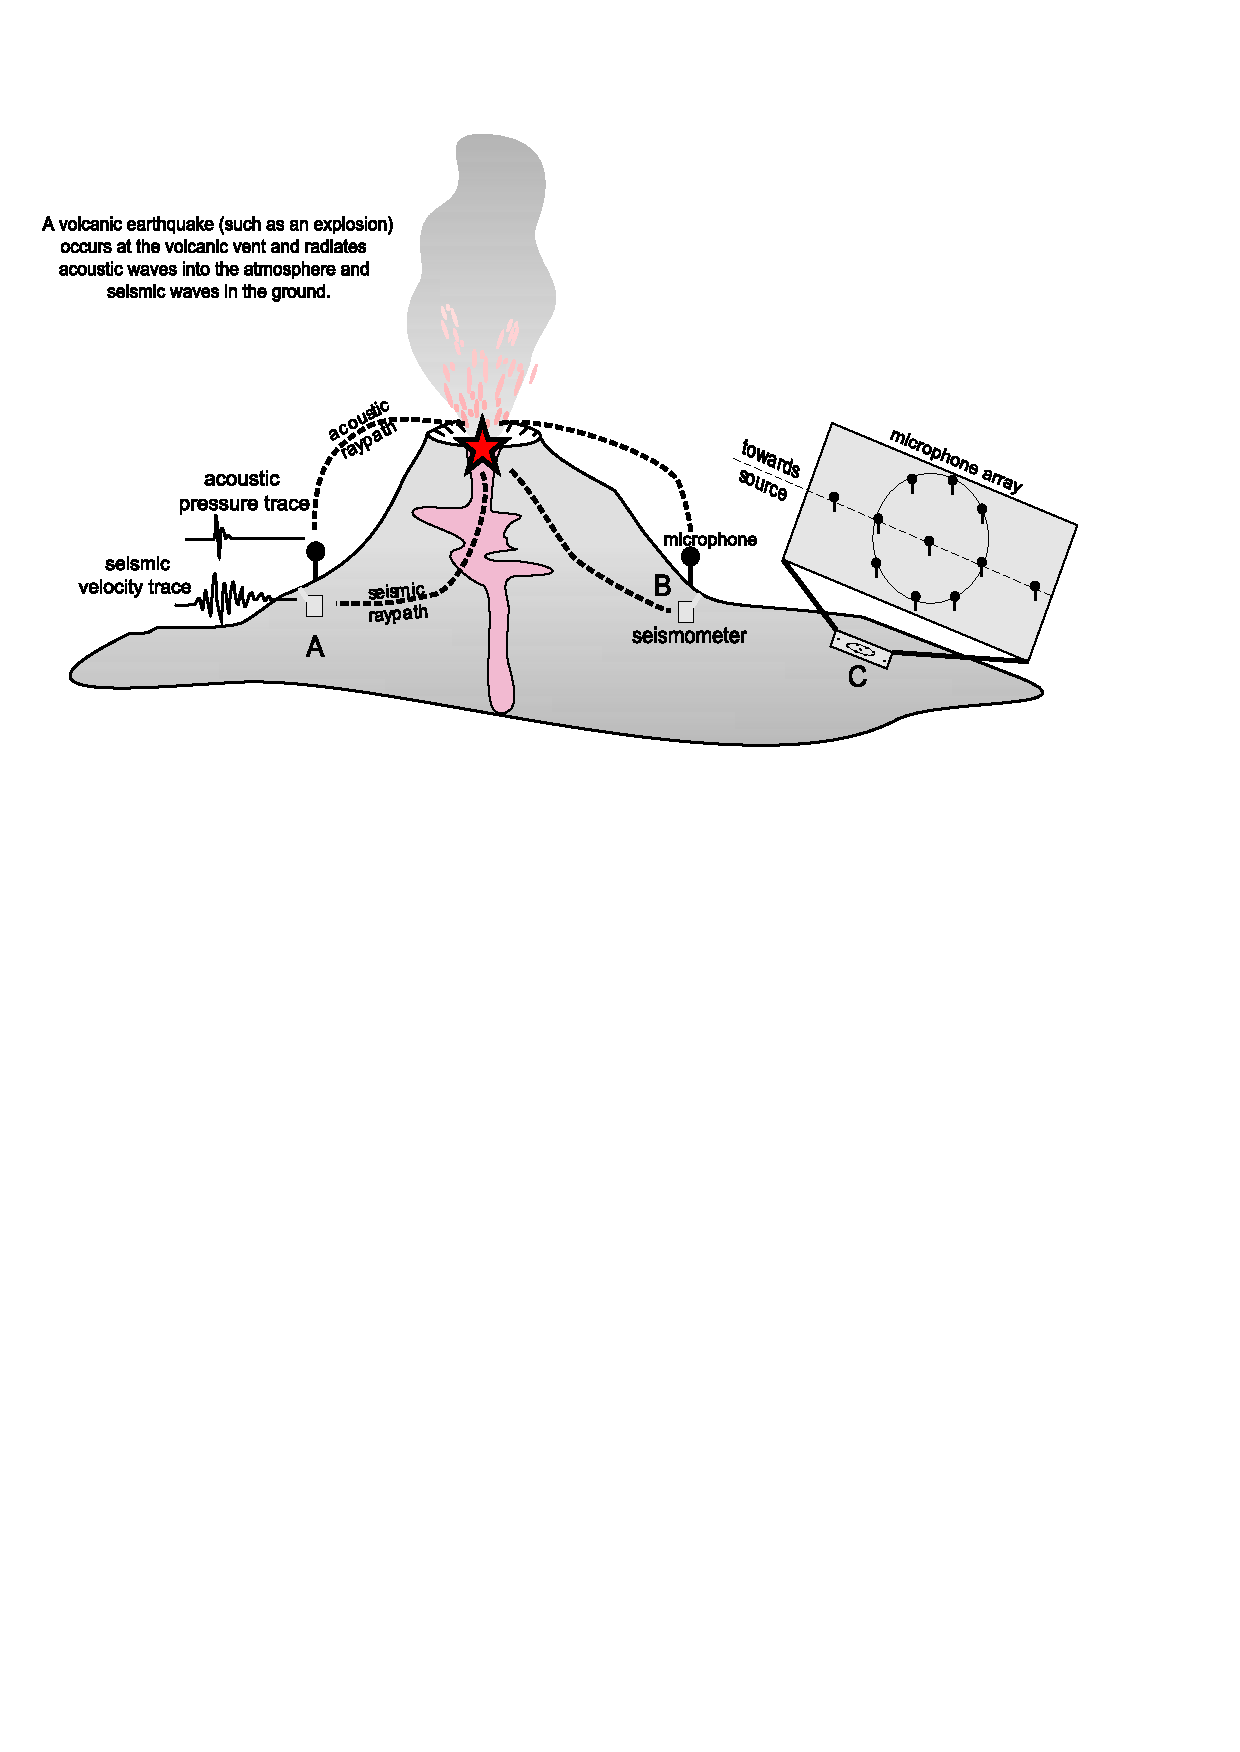
\includegraphics[width=0.9\hsize,clip=true,bb=20 470 540 770]{./figures/Cartoon2.pdf}
\end{center}
\caption{\small {\bf Sensor arrays for volcanic monitoring.}}
\label{fig-cartoon}
\end{figure*}

\subsection{Volcanic monitoring arrays and networks}

Volcanic sensors range from widely dispersed instrument networks to more
confined sensor arrays. An individual sensor station may consist of a
single sensor (e.g., seismometer or tilt sensor), or an array of several
closely-spaced ($10^2$ to $10^3$~m aperture) wired sensors, perhaps
of different types. Multiple stations may be integrated into a larger
network that is installed over an extended azimuthal distribution and
radial distance ($10^2$ to $10^4$~m) from the vent.  Data from the various
stations may be either recorded continuously or as triggered events and
the acquisition bandwidth depends upon the specific data stream. For
instance, seismic data is often acquired at 24-bit resolution at 100~Hz,
while tilt data may be recorded with 12-bit resolution at 1~Hz or less.

Sensor data at a station may be recorded locally or transmitted over
long-distance radio or telephone links to an observatory
located tens of kilometers from the volcano.  At the receiving site,
data is displayed on revolving paper helicorders for rapid general
interpretation and simultaneously digitized for further processing.
However, due to the expense and bandwidth constraints of radio telemetry,
high-quality, multi-channel data acquisition at a particular volcano is
often limited. These analog systems also suffer from signal degradation
and communication interference.

As a result, many scientific experiments use a stand-alone data
acquisition system at each recording station. 
The digitizer performs high-resolution 
analog-to-digital conversion from the wired sensors and stores data 
on a hard drive or Compact Flash card. However, these systems are
cumbersome, power hungry ($\approx
10$~Watts), and require data to be manually retrieved from the station
prior to processing. Depending on the size of the recording media,
a station may record several days or weeks' worth of data before
it must be serviced.

\subsection{Scientific and monitoring goals}

Volcanic monitoring has a wide range of goals, related to both
scientific studies and hazard monitoring. The type and configuration
of the instrumentation depends on the goals of a particular study.
Traditionally, dispersed networks of seismographs, which record 
ground-propagating elastic energy, are utilized to locate, determine the 
size of, and assess focal mechanisms (source motions) of earthquakes 
occurring within a volcanic edifice~\cite{Chouet03}. 
%Data from each 
%seismograph channel is usually recorded as a continuous time-series 
%of polarized local ground velocity.  
At least four 
spatially-distributed seismographs are required to constrain hypocentral 
(3D) source location and origin time of an earthquake, though
using more seismic elements enhances hypocenter resolution and the 
understanding of source mechanisms. Understanding spatial and temporal 
changes in the character of volcanic earthquakes is essential
for tracking volcanic activity, as well as predicting eruptions 
and paroxysmal events~\cite{McNutt96}. 

%well investigated through the 
%study of seismic network data and are critical for 

Another use of seismic networks is the imaging of the internal
structure of a volcano through tomographic inversion.  Earthquakes
recorded by spatially-distributed seismometers provide information
about propagation velocities between a particular source and receiver.
A seismically-active volcano thus allows for three-dimensional imaging
of the volcano's velocity structure~\cite{Benz96,Phillips91}. The
velocity structure can then be related to material properties of the
volcano, which may be used to determine the existence of a
magma chamber~\cite{Lees89,Moran99}.

Dense array configurations, with as many as several dozen
seismographs, are also an important focus of volcanic
research~\cite{Dietel89,Neuberg94}. Correlated seismic body and surface wave
phases can be tracked as they cross the array elements, enabling
particle motion and wavefield analysis, source back-azimuth calculations,
and enhanced signal-to-noise recovery.

\subsection{The role of infrasound}

Infrasonic signals are
becoming an increasingly important means by which to study volcanic
activity. An acoustic antenna, with three or more microphones that
record low-frequency sound pressure waves, are used for enhancing
signal-to-noise and discriminating the source of a volcanic
event~\cite{Johnson03}. In cases where the volcanic vent may not be
visible due to terrain or cloud cover, infrasonic signals can 
help differentiate eruptive activity from other sources of seismic 
signals such as mining operations or bovine ambulation. In volcanoes with multiple vents,
such as Stromboli, Italy, an array of acoustic sensors can
triangulate the precise location of individual eruptions~\cite{Ripepe02}.

Combining seismic and acoustic signals in a sensor array has great
potential for assessing eruption intensity and interpreting trends
in volcanic activity~\cite{Johnson04}.  Infrasonic signals have
also been used to track non-stationary sources~\cite{Yamasato97}
and to understand the weather-dependent velocity structure of the
atmosphere~\cite{Garces98}.

\subsection{Opportunities for wireless sensor networks}

Wireless sensor networks present new opportunities for volcanic
monitoring by offering increased scale and resolution.  As mentioned above,
analog radio telemetry has been used at volcanic monitoring stations
for some time. More recently, spread-spectrum digital modems have been
employed to transmit digital data from remote monitoring stations to an
observatory. For example, at Mount Erebus, Antarctica, a five-station
sensor array was installed that transmits real-time data over a FreeWave
modem~\cite{freewave} to a central PC that is connected to the Internet
over a geosynchronous satellite link~\cite{Aster04}.

However, these approaches are still limited in terms of the number of
individual channels (seismic, acoustic, etc.) that can be recorded at
each station and the communication bandwidth of the long-distance 
radio link. The number and placement of sensors at a station is limited by 
power requirements, cable length, and data recording capabilities.
For example, a typical data recorder supports only up to six 24-bit 
channels. The use of small, low-power, wireless sensor nodes can 
greatly benefit volcanic monitoring
studies, allowing researchers to deploy large sensor arrays in a
versatile fashion. A sensor array of tens of microphones or seismic
elements will improve spatial resolution and resilience to wind noise and
permit much more detailed analysis of received signals. Unlike a fixed data
logger, wireless sensor networks are 
reprogrammable, allowing researchers to experiment with signal processing,
compression, oversampling, and other techniques to improve the quality
of the data captured.

The use of wireless sensor networks in this context raises a number of
new challenges. The data rates from individual sensors ($\approx$ 100~Hz) 
are much higher than those in low data-rate applications, such as
environmental monitoring~\cite{mainwaring-habitat,gdi-ewsn04}. Therefore, new
approaches to managing bandwidth are required, since even a small 
number of sensors will saturate the wireless link. Rather than
sampling and transmitting data continuously, it is necessary to 
perform compression, correlation, or other processing of signals on
the sensor nodes themselves. In addition, sensor nodes must be tightly 
time synchronized to allow signals from each node to be compared. 


